\documentclass[10pt,twoside]{article}
\usepackage[utf8]{inputenc}
\usepackage{amsmath}
\usepackage{amsfonts}
\usepackage{amssymb}
\usepackage[spanish,es-noshorthands]{babel}
\usepackage[T1]{fontenc}
\usepackage{lmodern}
\usepackage{graphicx,hyperref}
\usepackage{tikz,pgf}
\usepackage{multicol}
\usepackage{subfig}
\usepackage[papersize={6.5in,8.5in},width=5.5in,height=7in]{geometry}
\usepackage{fancyhdr}
\pagestyle{fancy}
\fancyhead[LE]{
\includegraphics[height=12pt]{Images/logo-colegio.png} Aritmética $6^{\circ}$}
\fancyhead[RE]{}
\fancyhead[RO]{\textit{Germ\'an Avenda\~no Ram\'irez, Lic. U.D., M.Sc. U.N.}}
\fancyhead[LO]{}

\author{Germ\'an Avenda\~no Ram\'irez, Lic. U.D., M.Sc. U.N.}
\title{\begin{minipage}{.2\textwidth}

\includegraphics[height=1.75cm]{Images/logo-colegio.png}\end{minipage}
\begin{minipage}{.55\textwidth}
\begin{center}
Taller 12, Números primos  \\
Aritmética $6^{\circ}$
\end{center}
\end{minipage}\hfill
\begin{minipage}{.2\textwidth}

\includegraphics[height=1.75cm]{Images/logo-sed.png} 
\end{minipage}}
\date{}
\begin{document}
\maketitle
Nombre: \hrulefill Curso: \underline{\hspace*{44pt}} Fecha: \underline{\hspace*{2.5cm}}\\
\begin{enumerate}
 \item Construya los diagramas de árbol, para hallar los divisores de 36, de 100 y de 144
 \begin{enumerate}
  \item ¿Cuántos divisores tiene cada número?
  \item ¿Los divisores de un número son menores que él? ¿Por qué?
 \end{enumerate}
\item Sonia prepara para la venta, galletas de coco. Cada grupo de 24 galletas las empaca en cajas rectangulares, de manera que no sobren ni falten. ¿Cuáles son las posibles distribuciones que pueden hacer en las cajas para guardar las galletas?
\begin{center}
 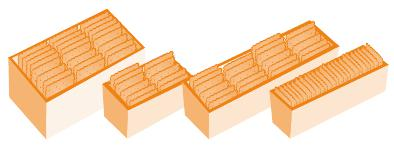
\includegraphics{../home/german/SparkleShare/My-repository/LaTeX/Images/galletas.jpg}
 % galletas.jpg: 394x147 pixel, 96dpi, 10.42x3.89 cm, bb=0 0 296 110
\end{center}

\end{enumerate}

\end{document}
